
\documentclass[]{emulateapj}
\usepackage{amsmath}

\usepackage[breaklinks,colorlinks,citecolor=blue,linkcolor=blue]{hyperref}
\usepackage{etoolbox}

\makeatletter

% Patch case where name and year are separated by aysep
\patchcmd{\NAT@citex}
  {\@citea\NAT@hyper@{%
     \NAT@nmfmt{\NAT@nm}%
     \hyper@natlinkbreak{\NAT@aysep\NAT@spacechar}{\@citeb\@extra@b@citeb}%
     \NAT@date}}
  {\@citea\NAT@nmfmt{\NAT@nm}%
   \NAT@aysep\NAT@spacechar\NAT@hyper@{\NAT@date}}{}{}

% Patch case where name and year are separated by opening bracket
\patchcmd{\NAT@citex}
  {\@citea\NAT@hyper@{%
     \NAT@nmfmt{\NAT@nm}%
     \hyper@natlinkbreak{\NAT@spacechar\NAT@@open\if*#1*\else#1\NAT@spacechar\fi}%
       {\@citeb\@extra@b@citeb}%
     \NAT@date}}
  {\@citea\NAT@nmfmt{\NAT@nm}%
   \NAT@spacechar\NAT@@open\if*#1*\else#1\NAT@spacechar\fi\NAT@hyper@{\NAT@date}}
  {}{}
  
\makeatother
%
\usepackage{xspace}
%
\usepackage{apjfonts}
\usepackage{amssymb, amsmath} % for e.g. \lesssim
\usepackage{natbibspacing, natbib}
\usepackage{aas_macros} % for understanding Journal in bib
\usepackage{graphics,graphicx}
%
\newcommand{\vdag}{(v)^\dagger}
\newcommand{\myemail}{tleung@astro.cornell.edu}
\newcommand{\Msun}{\mbox{$M_{\odot}$}\xspace}
\newcommand{\Rsun}{\mbox{$R_{\odot}$}\xspace}
\newcommand{\Lsun}{\mbox{$L_{\odot}$}\xspace}
\newcommand{\LIR}{\mbox{$L_{\rm IR}$}\xspace}
\newcommand{\LFIR}{\mbox{$L_{\rm FIR}$}\xspace}
%
\newcommand{\rarr}{$\rightarrow$}
\newcommand{\aco}{\mbox{CO($J$\,=\,1\,\rarr\,0) }}
\newcommand{\bco}{\mbox{CO($J$\,=\,2\,\rarr\,1) }}
\newcommand{\cco}{\mbox{CO($J$\,=\,3\,\rarr\,2) }}
\newcommand{\rot}[3][CO]{\mbox{#1($J$\,=\,#2\,\rarr\,#3)}}
%
\newcommand{\cii}{[C{\scriptsize II}]}
\newcommand{\Lp}[1][CO]{\mbox{$L^{\prime}_\textrm{\fontsize{8pt}{12pt}\selectfont{#1}}$}\xspace}
\newcommand{\kms}{\mbox{km\,s$^{-1}$}\xspace}
\newcommand{\LpU}{\mbox{K\,\,km\,\,s$^{-1}$\,\,pc$^2$}\xspace}
\newcommand{\pmOne}{\mbox{$^{-1}$}\xspace}
\newcommand{\alphaco}{\mbox{$\alpha_{\rm CO}$}\xspace}
\newcommand{\alphaU}{\mbox{$($K\,\,\kms\,\,pc$^2$$)$\pmOne}}
\newcommand{\sfrU}{\mbox{\Msun\,yr$^{-1}$}\xspace}
% Numerical values
\newcommand{\E}[1]{\mbox{$\times10^{#1}$}}
\newcommand{\petm}[2]{$^{+#1}_{-#2}$}
\newcommand{\eq}{\,=\,}
\newcommand{\pmm}{\,$\pm$\,}
%
\newcommand{\eg}{{e.g.,~}}
\newcommand{\ie}{{i.e.,~}}
%
\newcommand{\Fig}[1]{Figure~\ref{fig:#1}}
\newcommand{\Eq}[1]{Equation~\ref{eq:#1}}
\newcommand{\Tab}[1]{Table~\ref{tab:#1}}
\newcommand{\Sec}[1]{\S\ref{sec:#1}}
%
\newcommand\tna{\,\tablenotemark{a}}
\newcommand\tnb{\,\tablenotemark{b}}
\newcommand\tnc{\,\tablenotemark{c}}
\newcommand\tnd{\,\tablenotemark{d}}
\newcommand\tne{\,\tablenotemark{e}}
\newcommand\tnf{\,\tablenotemark{f}}
\newcommand\tng{\,\tablenotemark{g}}
\newcommand\tnh{\,\tablenotemark{h}}
\newcommand\tni{\,\tablenotemark{i}}
\newcommand\tnj{\,\tablenotemark{j}}
\newcommand\tnk{\,\tablenotemark{k}}
\newcommand\tnl{\,\tablenotemark{l}}
%
\def\herschel {{\it Herschel Space Observatory}\xspace}
\def\alma     {Atacama Large (sub-)Millimeter Array (ALMA)\xspace}
\def\spitzer {{\it Spitzer Space Telescope}\xspace}
\def\pdbi     {Plateau de Bure Interferometer\xspace}
\def\carma    {Combined Array for Research in Millimeter-wave Astronomy\xspace}
\def\cso      {Caltech Sumillimeter Observatory (CSO)\xspace}
\def\noema    {Northern Extended Millimeter Array (NOEMA)\xspace}
\def\vla      {{\it Karl G. Jansky} Very Large Array\xspace}
% Typography
\newcommand{\ncode}[1]{{\sc #1}}
% Codes / Softwares
\newcommand{\uvmcmcfit}{\ncode{uvmcmcfit}\xspace}
\def\aips {\ncode{AIPS}\xspace}
\def\casa {\ncode{CASA}\xspace}
% Long words
\newcommand{\lowZ}{low-metallicity\xspace}
\newcommand{\mulw}{multi-wavelength\xspace}
\newcommand{\SF}{star formation\xspace}
\newcommand{\SB}{starburst\xspace}
\newcommand{\SBs}{starbursts\xspace}
\newcommand{\gl}{gravitationally lensed\xspace}
\newcommand{\MCMC}{Markov Chain Monte Carlo (MCMC)\xspace}
% Wavelength regimes
\newcommand{\fir}{far-IR\xspace}
\newcommand{\fuv}{far-UV\xspace}
\newcommand{\mir}{mid-IR\xspace}
\newcommand{\nir}{near-IR\xspace}
\begin{document}
\author{Draft}


\section{Gravitational Lens model}

\subsection{interpretation}
- C06 suggest the presence of an interacting dusty galaxy in their HST
observations, which BJB+08 calls it the F component. The lensed images of the
ABCDE 
components coincide with our CO data (see mom0 on HST and channel map),
evidently CO emission coming from the AGN host galaxy. 
- one of the red channels in our lens model suggests a second source component,
which is consistent with the spatially offset dusty source (see mom0 on HST,
which 
the red velocity component coincides with this F component)

%%%%%%%%%%%%%%%%%%%%%%%%
+ Compare our lens model parameters on the mass distribution of the lensing
galaxy with literature (specifically SIE model in C06)
	- C06: SIE model shows position of lensing mass is offset by (-0.015",
-0.041" from obs. (i.e. light centroid)); PA = -73.6, ellipticity = 0.45,
theta\_R = 1.84" $\pm$ 0.01 
	- Our model lens parameters (median):
		- file: WRITEUP/MedianLensModelParams.txt
		- lensing gal. position is consistent with C06, 
		- Einstein radius: consistent with C06
		- PA: consistent within errors
		- Axial ratio: consistent within errors
%%%%%%%%%%%%%%%%%%%%%%%%%

\begin{deluxetable}{lcc}[!htbp]
\tabletypesize{\scriptsize}
\tablecolumns{3}
\tablecaption{Magnification factors of various kinematic components in \bco}
\tablehead{
\colhead{Velocity Range(\kms)} & % see 22May16/intensity30Apr16.spec; or channel map in paper
\colhead{Source 1 $\mu_{\rm L}$} &
\colhead{Source 2 $\mu_{\rm L}$}
}
\startdata
$-$366\,$-$\,$-$258 & 3.1 $\pm$ 0.9 & \\ [0.5ex]
$-$237\,$-$\,$-$151 & 4.3 $\pm$ 2.4 & \\ [0.5ex]
$-$129\,$-$\,$-$43  & 4.2 $\pm$ 0.6 & \\ [0.5ex]
$-$21.5\,$-$\,65    & 4.1 $\pm$ 0.9 & \\ [0.5ex]
86\,$-$\,172        & 8.7 $\pm$ 2.0 & \\ [0.5ex]
194\,$-$\,280       & 7.6 $\pm$ 1.6 & \\ [0.5ex]
301\,$-$\,388       & 7.2 $\pm$ 5.6 & 6.7 $\pm$ 2.5 \\ [0.5ex]
weighted average & 4.4 & \\ [0.5ex]
median & 5.5 &
\enddata
\label{tab:model}
\tablecomments{Velocity is taken from the center of each (native) channel
without any binning. Each row corresponds to a channel slice used for
lens modeling. Source 1 is RXJ1131 and source 2 is its companion. See text for details. }
\end{deluxetable}


\begin{figure}[tbph]
\centering
\includegraphics[width=0.50\textwidth]{../Figures/Pseudointegrated_datamodel.eps}
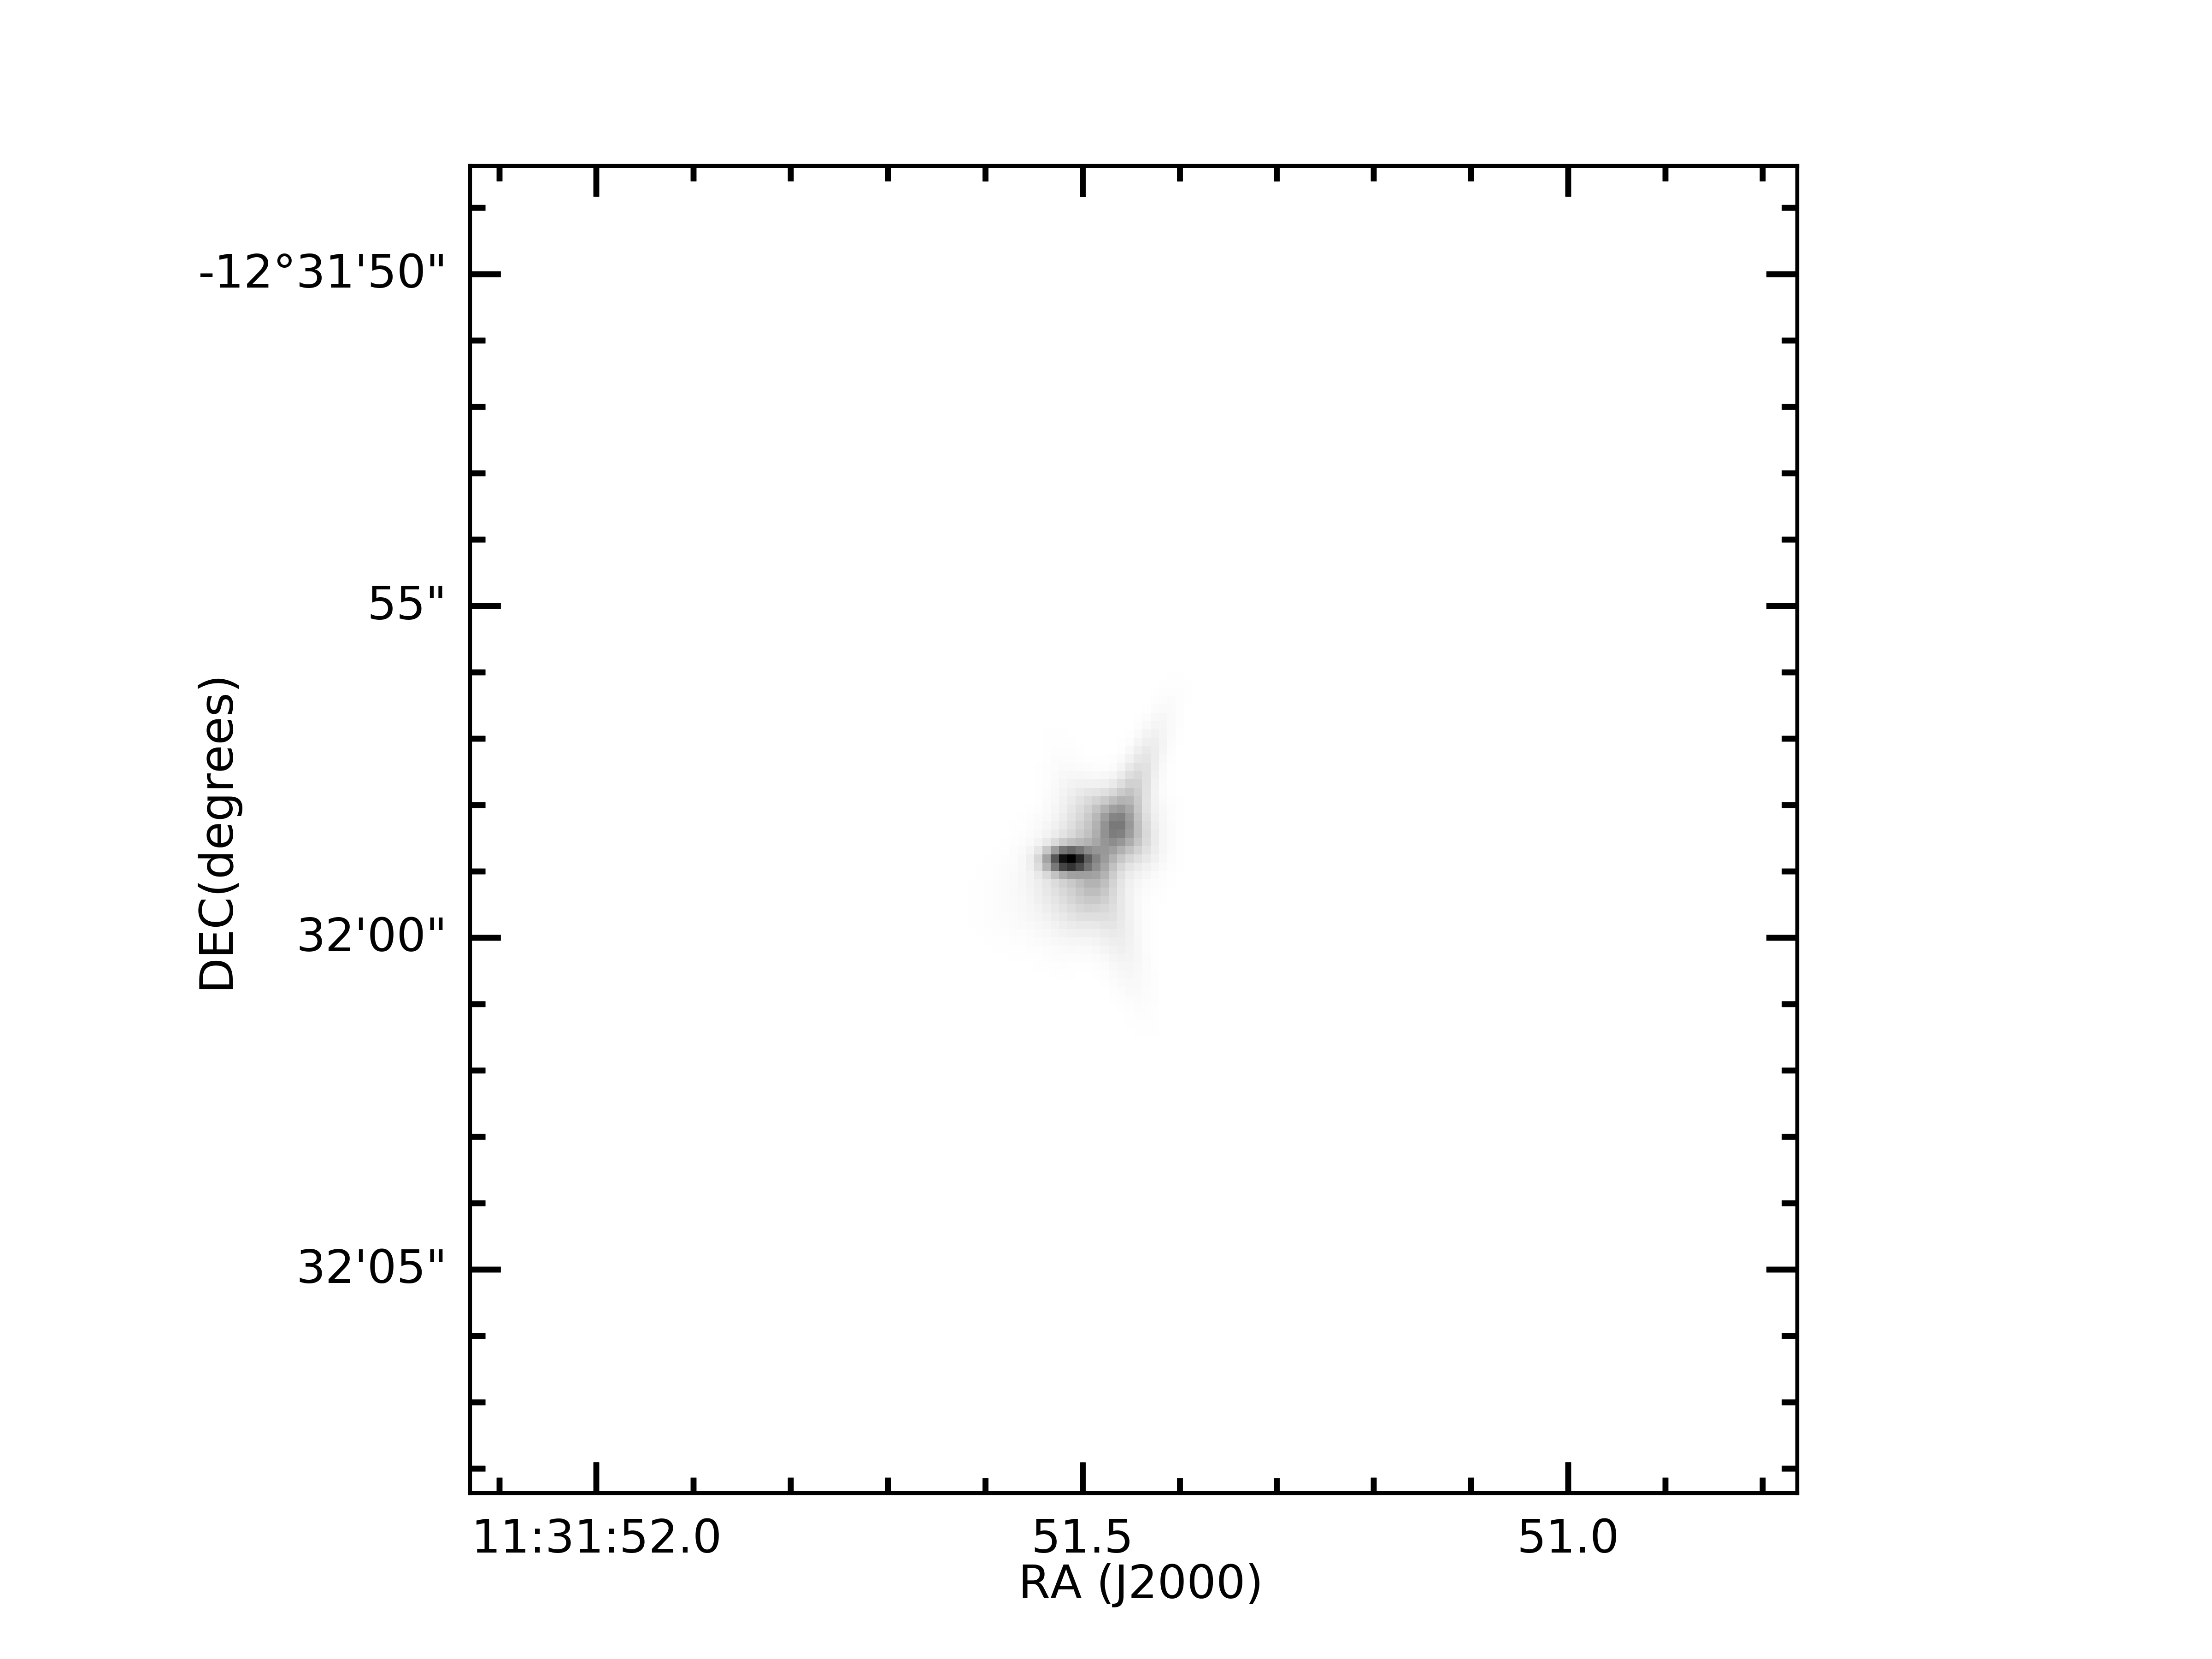
\includegraphics[width=0.50\textwidth]{../Figures/SourcesPlane.png}
\caption{
Pseudo observed 0th moment map in the lens plane. (left)
Pseudo 0th moment map in the source plane. (right)
\label{fig:}}
\end{figure}


%\begin{figure*}[tbph]
%\centering
%\caption{
%\label{fig:}}
%\end{figure*}


\begin{figure*}[tbph]
\centering
\includegraphics[width=0.80\textwidth]{../Figures/PseudoRGB_Lensed_SB_double.eps}
\caption{
velocity gradient of the lens model in the lens plane (left), source plane
(right).
\label{fig:}}
\end{figure*}


%\begin{figure*}[tbph]
%\centering
%\includegraphics[width=0.8\textwidth]{}
%\includegraphics[width=0.65\textwidth]{}
%\caption{
%\label{fig:}}
%\end{figure*}

\end{document}